
\titledquestion{Providing Counterexamples}
For each of the following statements, provide counterexamples by \textbf{drawing a graph and briefly explaining it} to illustrate that these three statements are incorrect.

\begin{parts}
    \part[3] Each DAG with $|V|$ vertices and $|V|-1$ edges has its unique topological sorting.
    \begin{solution}
        %\vspace{3.5cm}
        \\
        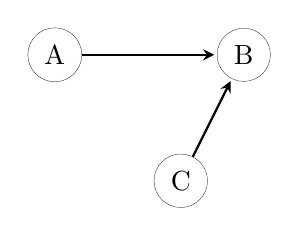
\begin{tikzpicture}[
            > = stealth, % arrow head style
            shorten > = 1pt, % don't touch arrow head to node
            node distance = 1cm, % distance between nodes
            thick, % line style
            scale = 0.8,
        ]
        \node[circle, draw, line width=0.1pt] (a) at (-3,3){A};
        \node[circle, draw, line width=0.1pt] (b) at (0, 3){B};
        \node[circle, draw, line width=0.1pt] (c) at (-1,1){C};
        \draw[->] (a) to (b);
        \draw[->] (c) to (b);
        \end{tikzpicture}
        \\
        it has two topological sorting results:\\
        $A,C,B$\\
        $C,A,B$
    \end{solution}
    \part[3] Since we can find a \textbf{maximum spanning tree} in a graph by multiplying all edge weights by $-1$ and then running Prim's algorithm, similarly we can find the \textbf{longest path} in a positive-weighted graph by negating all weights and running Dijkstra's algorithm from every source node.
    \begin{solution}
        % \vspace{4cm}
        \\\\
        \begin{tikzpicture}[
            > = stealth, % arrow head style
            shorten > = 1pt, % don't touch arrow head to node
            node distance = 1cm, % distance between nodes
            thick, % line style
            scale = 0.8,
        ]
        \node[circle, draw, line width=0.1pt] (a) at (-3,2){A};
        \node[circle, draw, line width=0.1pt] (b) at (0, 2){B};
        \node[circle, draw, line width=0.1pt] (c) at (-1.5,-0.5){C};
        \draw[->] (a) to node[up]{2} (b);
        \draw[->] (a) to node[left]{1} (c);
        \draw[->] (c) to node[right]{3} (b);
        \end{tikzpicture}
        \\
        if we set the source node be $A$, the terminal node be $B$, then after nagating all weights, the graph become\\\\
        \begin{tikzpicture}[
            > = stealth, % arrow head style
            shorten > = 1pt, % don't touch arrow head to node
            node distance = 1cm, % distance between nodes
            thick, % line style
            scale = 0.8,
        ]
        \node[circle, draw, line width=0.1pt] (a) at (-3,2){A};
        \node[circle, draw, line width=0.1pt] (b) at (0, 2){B};
        \node[circle, draw, line width=0.1pt] (c) at (-1.5,-0.5){C};
        \draw[->] (a) to node[up]{-2} (b);
        \draw[->] (a) to node[left]{-1} (c);
        \draw[->] (c) to node[right]{-3} (b);
        \end{tikzpicture}
        \\And when running Dijkstra's algorithm on the new graph from source node $A$, end at terminal node $B$.\\
        after the first time, node $B$ has the weight $-2$, which is less than $C$'s $-1$, so we will mark node $B$ as visited,
        and the final weight from $A$ to $B$ become $-2$, however, the shortest path on the new graph from $A$ to $B$ should be $-4$.
        so it is incorrect.\\
        $i.e.$ after negating all weights and running Dijkstra’s algorithm, we get the longest path $2$, however, it should be $4$.


    \end{solution}
    \newpage
    \part[3] Assume that we implement Dijkstra’s algorithm with a binary heap as the priority queue in a positive-weighted graph, then we can do the following operation: when the terminal vertex is pushed into the priority queue, we can stop the algorithm and return the correct shortest path from the source vertex to the terminal vertex, instead of keeping running the algorithm until popping the terminal vertex from the heap.
    \begin{solution}
        % \vspace{4cm}
        \\\\
        \begin{tikzpicture}[
            > = stealth, % arrow head style
            shorten > = 1pt, % don't touch arrow head to node
            node distance = 1cm, % distance between nodes
            thick, % line style
            scale = 0.8,
        ]
        \node[circle, draw, line width=0.1pt] (a) at (-3,2){A};
        \node[circle, draw, line width=0.1pt] (b) at (0, 2){B};
        \node[circle, draw, line width=0.1pt] (c) at (-1.5,-0.5){C};
        \draw[->] (a) to node[up]{10} (b);
        \draw[->] (a) to node[left]{1} (c);
        \draw[->] (c) to node[right]{1} (b);
        \end{tikzpicture}
        \\
        if we set the source node be $A$, the terminal node be $B$, then\\
        if stop the algorithm when pushed the terminal node into the priority queue, then the result is :\\
        the path is $A\to B$, and the total weight is $10$.\\
        but if stop the algorithm when popping the terminal node into the priority queue, then the result is :\\
        the path is $A\to C\to B$, and the total weight is $2$. which is better than the previous one.\\
        

    \end{solution}
\end{parts}